% \documentclass[twocolumn]{article}

\documentclass{article}
\usepackage{graphicx} % Required for inserting images
\usepackage{url}
\usepackage{array} % Needed for custom column specifier
\usepackage{array} % Needed for custom column specifier
\usepackage{changepage} % Needed for adjustwidth environment
\usepackage{float}

\title{Topographical Scalp Maps for Hearing Impairment Detection: A CNN Approach
}
\author{Grace Wang, Dr. Beiyu Lin }
\date{July 2023}

\begin{document}

\maketitle

\section{Abstract}
It is estimated that more than $50\%$ of people over the age of 65 experience some form of hearing loss. The goal of this project is to utilize scalp maps derived from spatial and temporal electroencephalography (EEG) data to distinguish between individuals with hearing impairment and healthy individuals. A CNN model will be trained to recognize patterns in the spatial and temporal EEG data that can accurately classify the two groups. After experimenting with the CNN model and data splits, the model achieves an accuracy of $85\%-95\%$. The use of advanced technology like CNNs can potentially lead to more efficient and accurate hearing impairment detection methods, benefiting individuals and healthcare professionals alike.

\section{Introduction}
The normal hearing threshold for healthy individuals is 0 to 20 dB. A person is said to be hearing impaired if their hearing threshold is greater than 35 decibels (dB) in the better hearing ear. This means it becomes challenging for the affected individual to communicate without the use of hearing aids or assistive devices.

Current diagnostic methods, such as otoacoustic emission testing, MRI scans, and CT scans, assist in distinguishing between healthy individuals and those with hearing loss. However, this study explores an alternative approach by utilizing scalp maps derived from spatial and temporal EEG data, which records the brain's electrical activity through electrodes on the scalp. EEG offers affordability and non-invasiveness, making it a valuable tool in studying brain activity, cognitive processes, and neurological disorders. A deep learning model based on CNNs is employed due to its image-based nature, ideally suited for the visual nature of scalp maps. The potential of CNNs in hearing impairment detection could lead to earlier intervention and cost savings in healthcare by minimizing the need for extensive treatments resulting from untreated hearing loss.

\section{Terminologies}

\begin{itemize}
  \item \textit{EEG (Electroencephalography):} EEG is a technique used to record the electrical activity of the brain. It measures the electrical potentials generated by the brain's neurons through electrodes placed on the scalp.
  
  \item \textit{ERPs (Event-Related Potentials):} ERPs are specific components of the EEG signal that are time-locked to a particular event or stimulus, such as the presentation of a tone or visual stimulus. ERPs represent the brain's electrical response to these specific events and are characterized by distinct waveforms.
  
  \item \textit{Scalp Maps:} Scalp maps, also known as topographical maps, are graphical representations of the spatial distribution of brain electrical activity recorded by EEG electrodes on the scalp. They provide a visual depiction of the magnitude and location of brain activity at specific time points or time intervals.
  
  \item \textit{Spatial EEG Data:} Spatial EEG data refers to the patterns of electrical activity across different regions of the scalp. These patterns can be analyzed to identify brain regions involved in specific cognitive processes or responses to stimuli.
  
  \item \textit{Temporal EEG Data:} Temporal EEG data refers to the patterns of electrical activity over time. It captures the dynamic changes in brain activity in response to events or stimuli.
  
  \item \textit{EEG Preprocessing:} EEG preprocessing involves data cleaning and enhancement steps to remove noise, artifacts, and other sources of interference from the raw EEG signals. Common preprocessing steps include filtering, artifact removal, and baseline correction.
  
  \item \textit{Feature Extraction:} Feature extraction is the process of identifying and extracting relevant features from the ERP waveforms. These features capture important characteristics of brain activity and are used as input to machine learning models for classification tasks.
\end{itemize}

\section{Database}
In this study, we used a dataset containing EEG of 22 hearing impaired (HI) listeners with sensorineural hearing loss and 22 age matched normal hearing (NH) peers (between 51 - 76 years old). The data was collected from a previous study by Fuglsang et al. (2020). For this study, we are specifically looking at the tone stimuli experiment where during passive listening, event-related potentials (ERPs) were recorded while subjects were exposed to 1 kHz pure tones. These tones had a duration of 100 ms and were smoothly ramped using a 10 ms Hann window. The presentation rate of the tones was around 1 second on average, with random fluctuations of up to ±25 ms (jittered). Each subject underwent 180 repetitions of the tone stimuli.

\section{Methods}
The study consists of 4 main parts, including EEG signal processing, ERP extraction, extracting topographic brain maps, and training, validating, and testing the model. The first part includes EEG signal preprocessing and extraction of event-related potential features, which are used to draw the topographic brain map. 

\subsection{EEG Preprocessing}
EEG preprocessing and most of the ERP extraction were already completed by the researchers of the dataset. The explanation for how they preprocessed and extracted ERP is detailed in the paper, and the repository that contains code for the analysis of auditory EEG data is located at \url{https://gitlab.com/sfugl/snhl}. 

\subsection{ERP Extraction}
In the additional figures section of the repository at the bottom of the 'project overview,' Fig S2 contains a graph of the individual traces of ERP data averaged over the fronto-central electrode cluster, and the thin lines reflect the data from individual subjects. Thick lines show group mean averages. Within the repository, there is a script that calculates the mean average lines within the \texttt{snhl/reports/paper/func/extract\_erp.m} file path. 

\begin{figure}[H]
  \centering
  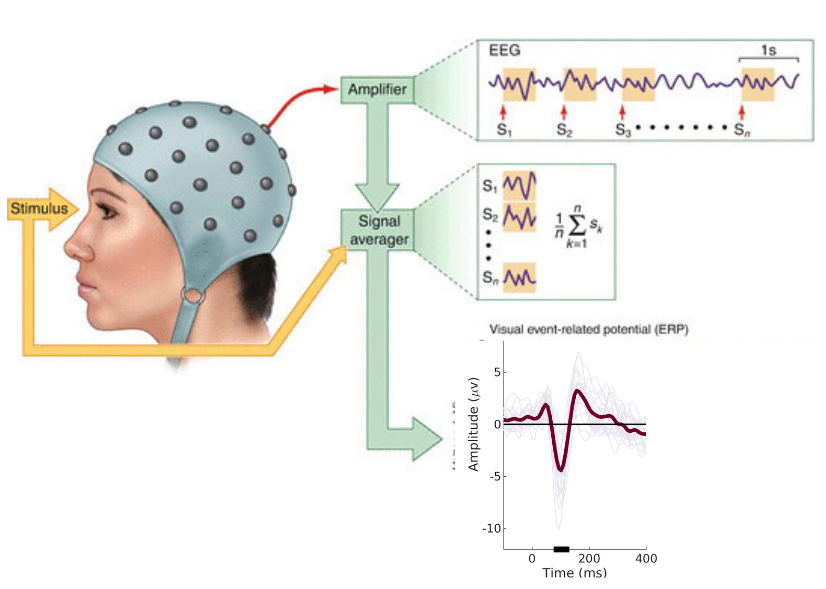
\includegraphics[width=1\textwidth]{Untitled design.png} % Replace "averaging.jpg" with the actual filename of your image
  \caption{Visual representation of how ERPs are derived from EEG data.} % Add your caption here
  \label{fig:averaging} % Add a label for referencing the figure in your text (optional)
\end{figure}

\begin{figure}[H]
  \centering
  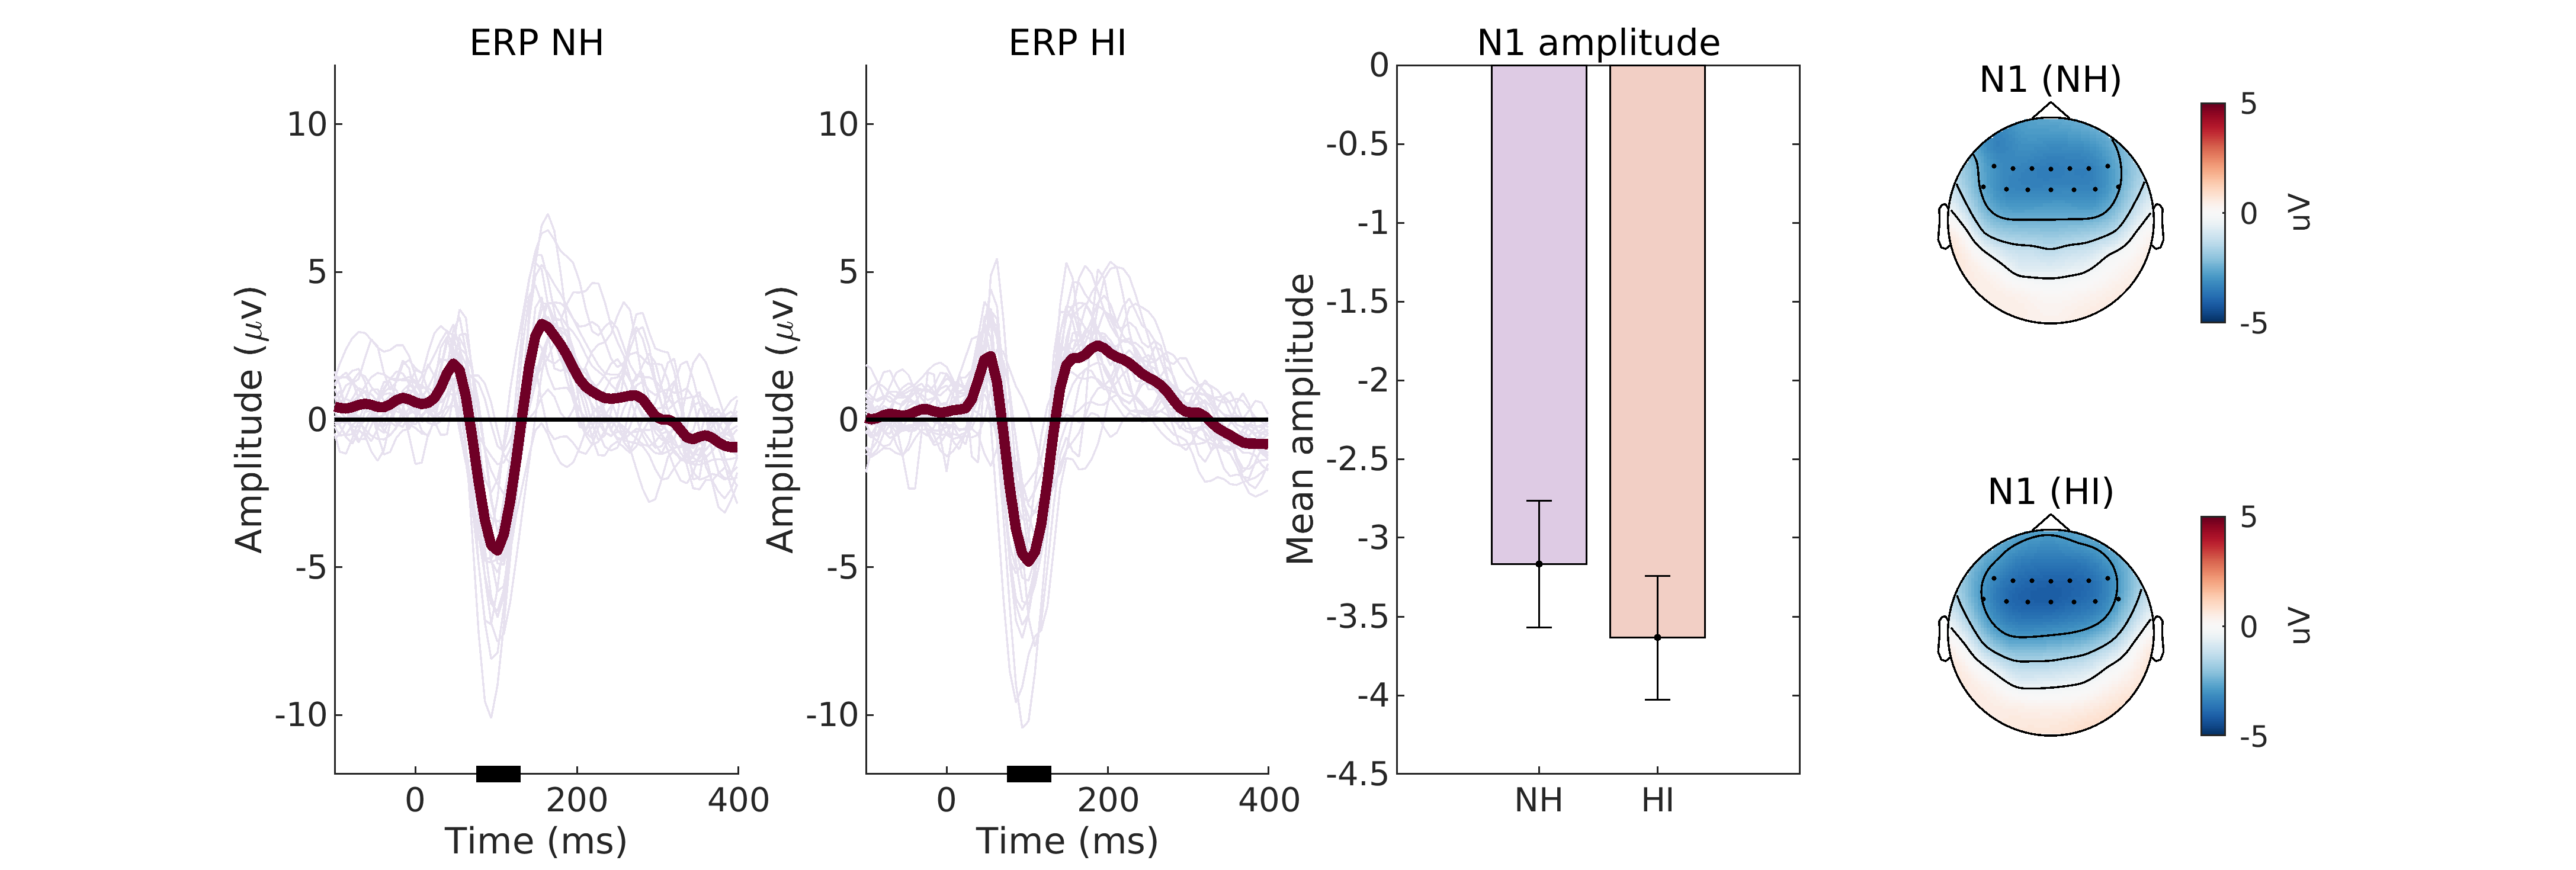
\includegraphics[width=1\textwidth]{figure-erp.png} % Replace "averaging.jpg" with the actual filename of your image
  \caption{First and second panel (from left): Individual traces of ERP data averaged over the same fronto-central electrode cluster that was used for the entrainment analysis. Thin lines reflect data from individual subjects. Thick lines reflect group-mean averages. Third panel: Mean amplitude of N1 ERPs averaged over a time interval from 75 ms to 130 ms. Errorbars show s.e.m. across listeners. Fourth (right) panel: Group-mean topographies of mean N1 amplitude.
} % Add your caption here
  \label{fig:erp} % Add a label for referencing the figure in your text (optional)
\end{figure}

\subsection{Topographic Brain Maps}
ERPs are the features we are using to classify the two groups. Given each patient's ERP waveform, which was up to 400 ms after the onset of tone stimuli, we created a matlab script to loop through each patient's individual ERP and extracted topographical scalp maps at every 10 ms intervals from 0 to 400 ms, giving us 40 scalp maps per subject. This results in a total of 1,760 images for our CNN model, with 44 subjects and 40 images each.
\begin{figure}[H]
  \centering
  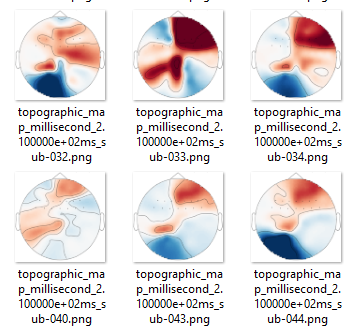
\includegraphics[width=0.8\textwidth]{scalpmaps.png} % Replace "averaging.jpg" with the actual filename of your image
  \caption{Examples of scalp maps} % Add your caption here
\end{figure}

\subsection{Convolutional Neural Network (CNN) Architecture}
We employed a CNN model to perform image classification on the dataset. The CNN model was implemented using the TensorFlow Keras library in a python notebook. The architecture consists of three convolutional layers, each followed by a max-pooling layer to extract relevant features from the input images. Specifically, the layers had filter sizes of 32, 64, 128, respectively with a ReLU activation function applied after each convolutional layer. Max-pooling layers with a 2x2 kernel were used to downsample the feature maps. The final layers included a flatten layer followed by a fully connected dense layer with 512 units and a ReLU activation function. A dropout layer with a dropout rate of 0.5 was applied to mitigate overfitting. The output layer consists of two units representing the two classes (Hearing Impaired and Healthy), with a softmax activation function to predict the probability distribution of each class.
\begin{figure}[H]
  \centering
  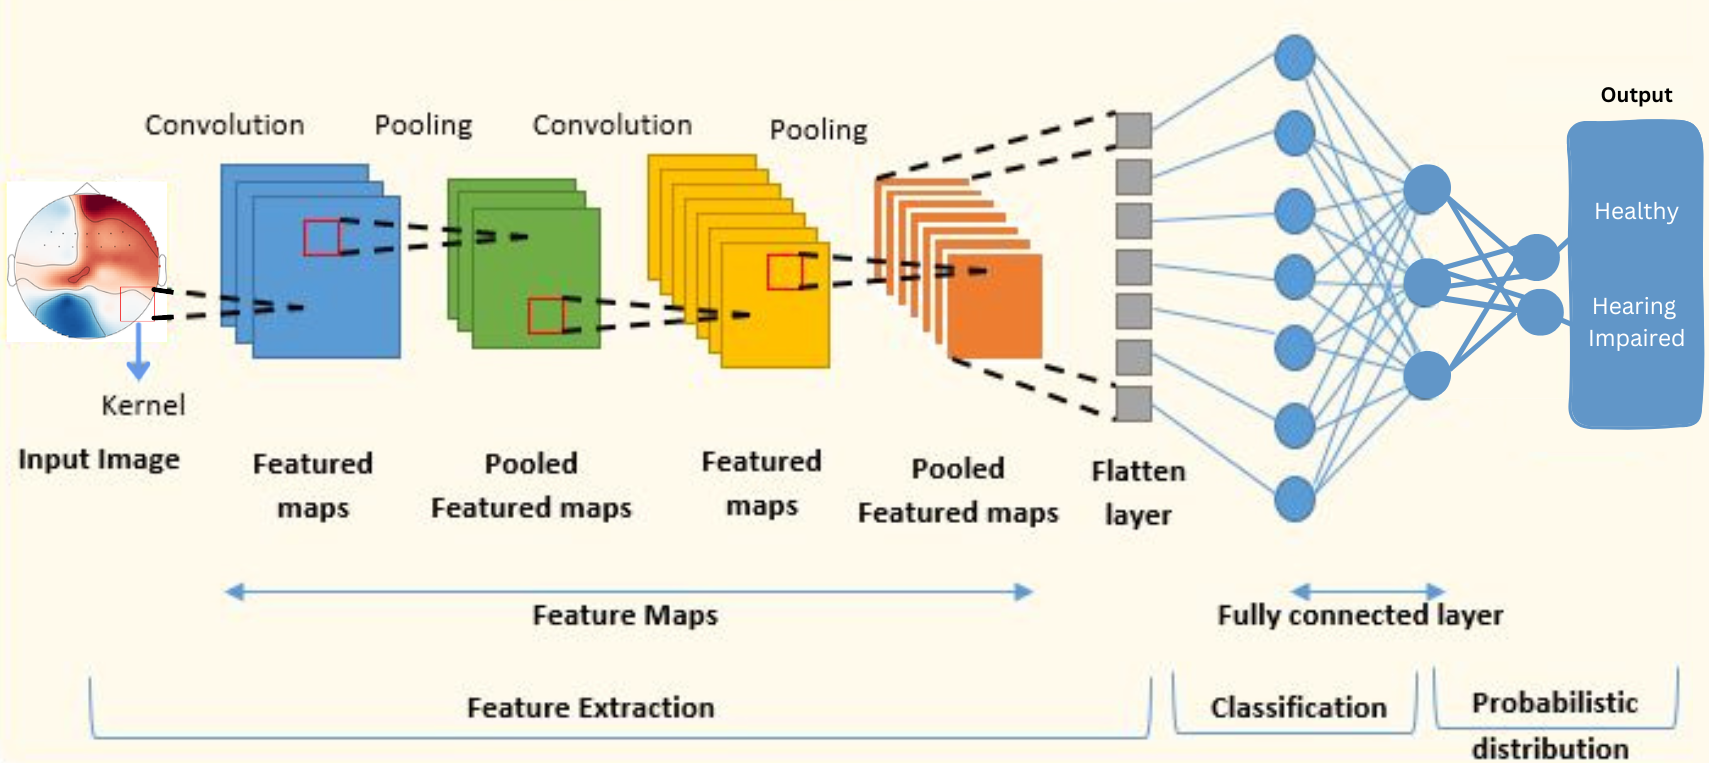
\includegraphics[width=1\textwidth]{Add a subheading.png} % Replace "averaging.jpg" with the actual filename of your image
  \caption{visual representation of CNN model} % Add your caption here
\end{figure}

\section{Results}

\subsection{Experiments}
Due to the limited size of our dataset, consisting of only 1,760 total images, we conducted various experiments to determine the most suitable division of data for training, validation, and testing purposes. As a result of these experiments, we obtained varying test accuracies.

\subsubsection{Experiment 1: 70\% Training, 30\% Testing}
\begin{table}[ht]
  \centering
  \caption{Classification Report (Experiment 1)}
  \label{tab:classification_report_1}
  \begin{tabular}{lcccc}
    \hline
    & Precision & Recall & F1-score & Support \\
    \hline
    Healthy & 0.86 & 0.86 & 0.86 & 264 \\
    Hearing Impaired & 0.86 & 0.86 & 0.86 & 264 \\
    \hline
    Accuracy & & & 0.86 & 528 \\
    Macro Avg & 0.86 & 0.86 & 0.86 & 528 \\
    Weighted Avg & 0.86 & 0.86 & 0.86 & 528 \\
    \hline
  \end{tabular}
\end{table}

\subsubsection{Experiment 2: 80\% Training, 10\% Validation, 10\% Testing}
\begin{table}[ht]
  \centering
  \caption{Classification Report (Experiment 2)}
  \label{tab:classification_report_2}
  \begin{tabular}{lcccc}
    \hline
    & Precision & Recall & F1-score & Support \\
    \hline
    Healthy & 0.98 & 0.92 & 0.95 & 88 \\
    Hearing Impaired & 0.92 & 0.98 & 0.95 & 88 \\
    \hline
    Accuracy & & & 0.95 & 176 \\
    Macro Avg & 0.95 & 0.95 & 0.95 & 176 \\
    Weighted Avg & 0.95 & 0.95 & 0.95 & 176 \\
    \hline
  \end{tabular}
\end{table}

\begin{figure}[H]
  \centering
  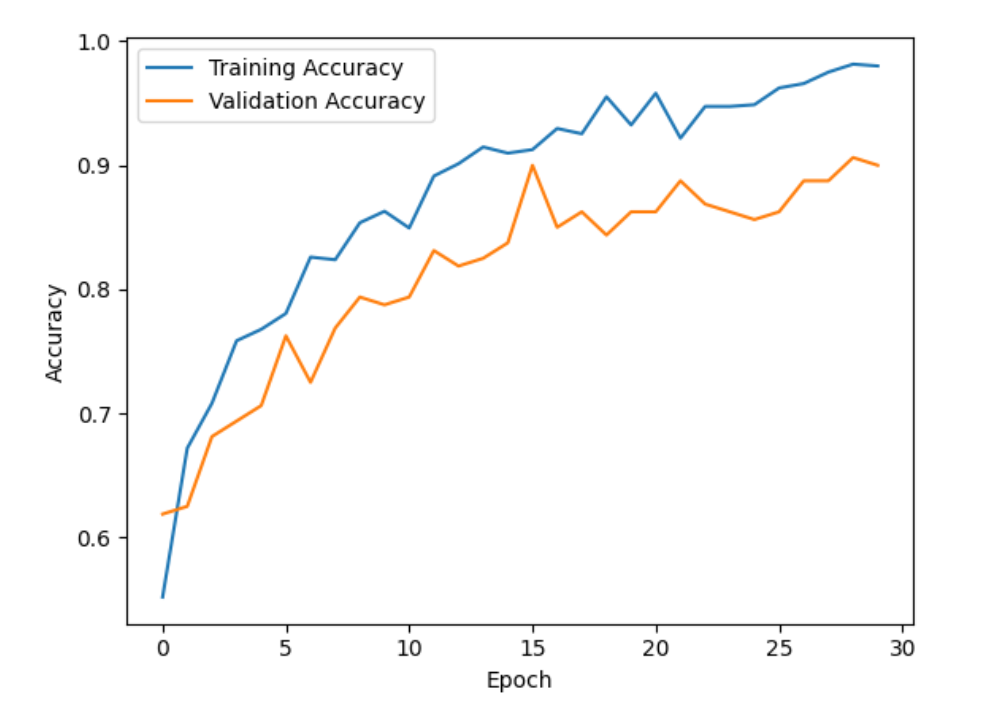
\includegraphics[width=0.7\textwidth]{801010.png} % Replace "801010.png" with the actual filename of your image
  \caption{Accuracy of Trained CNN Model}
  \label{fig:accuracy_cnn}
\end{figure}


\subsubsection{Experiment 3: 70\% Training, 15\% Validation, 15\% Testing}
\begin{table}[H]
  \centering
  \caption{Classification Report (Experiment 3)}
  \label{tab:classification_report_3}
  \begin{tabular}{lcccc}
    \hline
    & Precision & Recall & F1-score & Support \\
    \hline
    Healthy & 0.90 & 0.88 & 0.89 & 132 \\
    Hearing Impaired & 0.88 & 0.90 & 0.89 & 132 \\
    \hline
    Accuracy & & & 0.89 & 264 \\
    Macro Avg & 0.89 & 0.89 & 0.89 & 264 \\
    Weighted Avg & 0.89 & 0.89 & 0.89 & 264 \\
    \hline
  \end{tabular}
\end{table}

\begin{figure}[H]
  \centering
  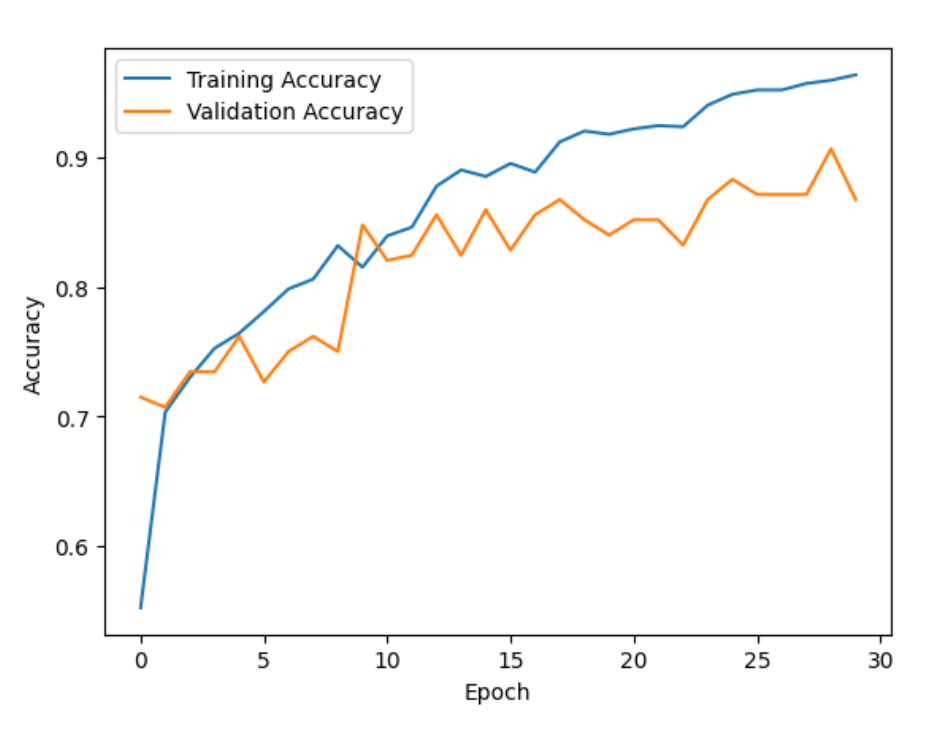
\includegraphics[width=0.7\textwidth]{701515.png} % Replace "801010.png" with the actual filename of your image
  \caption{Accuracy of Trained CNN Model}
  \label{fig:accuracy_cnn}
\end{figure}

\subsection{Experiments Summary}

\begin{table}[ht]
  \centering
  \caption{Experiment Results}
  \label{tab:experiment}
  % \small % Smaller font size
  \setlength{\tabcolsep}{6pt} % Adjust column width
  \begin{tabular}{|c|c|c|c|c|c|}
    \hline
    \textbf{Experiment} & \textbf{Training Data} & \textbf{Validation Data} & \textbf{Testing Data} & \textbf{Test Loss} & \textbf{Test Accuracy} \\
    \hline
    1 & 70\% & -- & 30\% & 0.379 & 0.865 \\
    \hline
    2 & 80\% & 10\% & 10\% & 0.227 & 0.950 \\
    \hline
    3 & 70\% & 15\% & 15\% & 0.470 & 0.891 \\
    \hline
  \end{tabular}
\end{table}



\section{Conclusions}
The CNN architecture employed in this study achieves a satisfactory performance of approximately 85\%-95\% accuracy in distinguishing between individuals with hearing impairment and healthy individuals based on scalp maps derived from spatial and temporal EEG data.

\section{Future Work}
For future investigations, several important steps can be taken to further enhance the model's accuracy and generalization. Firstly, applying this model on a different and larger dataset would be beneficial to assess its performance in a more diverse population. A larger dataset can help validate the model's effectiveness and robustness across a broader range of individuals.

Moreover, exploring alternative machine learning methods beyond CNNs, such as support vector machines (SVM), random forests, or recurrent neural networks (RNNs), could offer valuable insights and potentially lead to even higher accuracies. Comparing the performance of different machine learning algorithms can provide a better understanding of which approach is most suitable for this specific classification task.

Additionally, fine-tuning the model parameters and conducting necessary optimizations can significantly improve its performance. Techniques like cross-validation, hyperparameter tuning, and regularization can be employed to fine-tune the model, ensuring it is well-optimized and less prone to overfitting.

\section{References}
\section{Acknowledgments}

% \begin{table}[ht]
%     \centering
%     \begin{tabular}{cc}
%        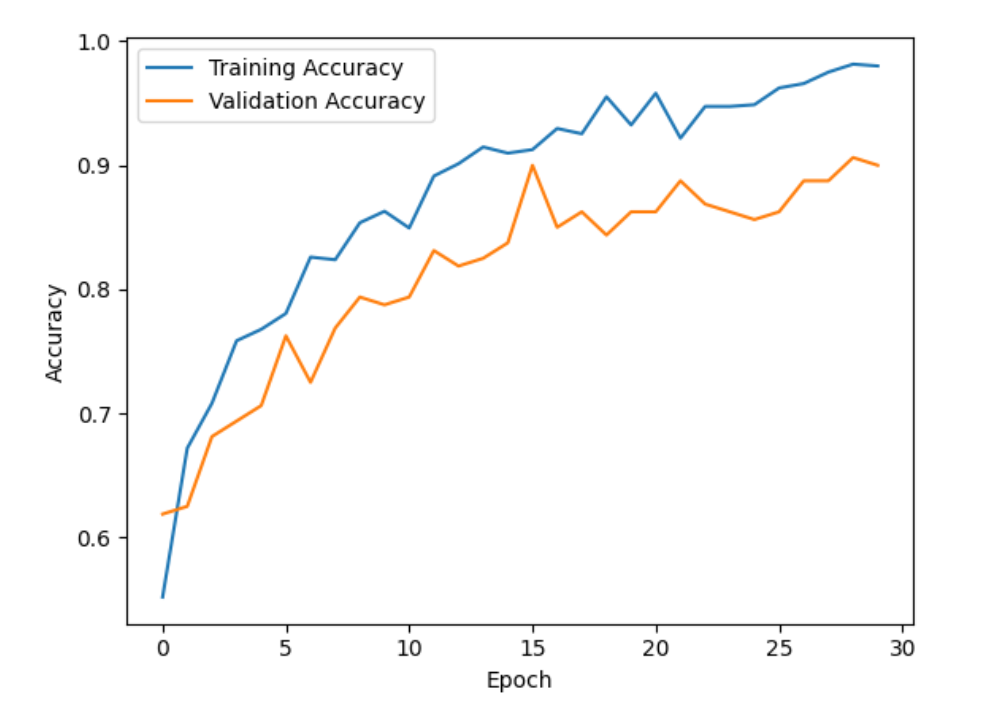
\includegraphics[width=0.43\linewidth]{801010.png} &
%         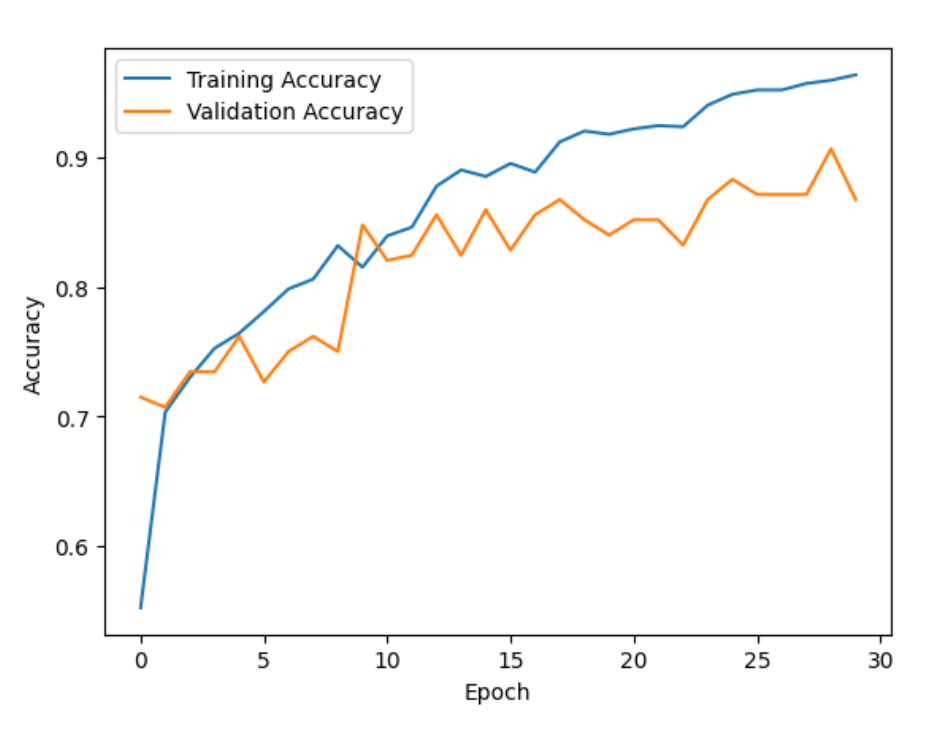
\includegraphics[width=0.4\linewidth]{701515.png} \\
%         Fig. 1: Learning curve (Experiment 1) & Fig. 2: Learning curve (Experiment 2) \\
%     \end{tabular}
%     \caption{Table of Images}
%     \label{tab:images}
% \end{table}

\end{document}




